\documentclass[tikz]{standalone}
\usepackage{pgfplots}
\pgfplotsset{compat=1.15}
\usepackage{mathrsfs}
\usetikzlibrary{arrows,calc}
\usepackage{tkz-euclide}

\usepackage{fp}
\pagestyle{empty}

\definecolor{AngleClr}{rgb}{0,0.39215686274509803,0}
\definecolor{ShapeClr}{rgb}{0.6,0.2,0}

\begin{document}

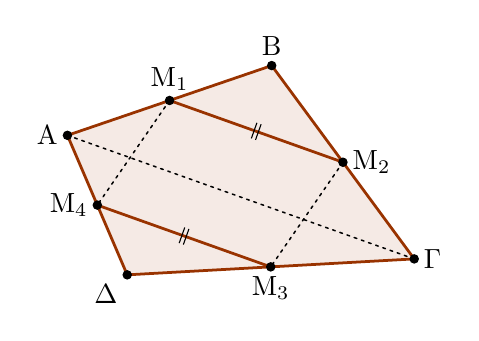
\begin{tikzpicture}[scale=.75]
\tkzSetUpLine[line width=1pt,color=black]
\tkzSetUpPoint[fill=black]

\def\Scale{1.35}
\FPeval{\Ax}{1.25 * \Scale}
\FPeval{\Ay}{3.6 * \Scale}
\FPeval{\Cx}{2.1 * \Ax}
\FPeval{\Ccx}{0.2 * \Scale}
\FPeval{\Cy}{1.45 * \Ax}
\FPeval{\Dx}{1.40 * \Ax}
\FPeval{\Dy}{(-1) * 0.6 * \Ax}

\tkzDefPoints{0/0/D,\Ay/\Ccx/C,\Cy/\Cx/B,\Dy/\Dx/A}

\tkzDefMidPoint(A,B) \tkzGetPoint{M1}
\tkzDefMidPoint(B,C) \tkzGetPoint{M2}
\tkzDefMidPoint(C,D) \tkzGetPoint{M3}
\tkzDefMidPoint(D,A) \tkzGetPoint{M4}


\tkzFillPolygon[fill=ShapeClr,fill opacity=0.1](A,B,C,D)

\tkzDrawSegments[line width=0.55pt,color=black,dashed,dash pattern=on 1pt off 1.75pt](A,C M1,M4 M2,M3)
\tkzDrawSegments[color=ShapeClr](M1,M2 M3,M4)

\tkzDrawPolygon[color=ShapeClr](A,B,C,D)
\tkzDrawPoints[size=3](A,B,C,D,M1,M2,M3,M4)
\tkzLabelPoint[left](A){$\rm A$}
\tkzLabelPoint[above](B){$\rm B$}
\tkzLabelPoint[right](C){$\rm \Gamma$}
\tkzLabelPoint[below left](D){$\rm \Delta$}

\tkzLabelPoint[above](M1){$\rm M_1$}
\tkzLabelPoint[right](M2){$\rm M_2$}
\tkzLabelPoint[below](M3){$\rm M_3$}
\tkzLabelPoint[left](M4){$\rm M_4$}


\tkzMarkSegments[mark=||,size=3](M1,M2 M3,M4)

\end{tikzpicture}

\end{document}
